\onecolumn
\clearpage
\renewcommand{\thetable}{A\arabic{table}}
\renewcommand\thesection{\Alph{section}}
\setcounter{section}{0}
{
\centering
\Large
\textbf{Can Natural Image Autoencoders Compactly Tokenize fMRI Volumes \\for Long-Range Dynamics Modeling?}\\
\vspace{0.5em}Appendix\\
\vspace{1.0em}
}

\section{Implementation Details}
\label{sec:experimental_details}
For the 2D DCAE, we brought the unmodified \texttt{dc-ae-f32c32-in-1.0} checkpoint provided by \citet{DCAE} for all 2D natural image DCAE experiments.

All experiments were conducted on the NVIDIA A100-40GB and RTX A6000 GPUs. We used \texttt{fp16} mixed precision for the training of all models except for TFF due to NaN error during training.

We used \texttt{BCEWithLogitsLoss} for the classification task, and used \texttt{pos-weight} option for the ADHD task to account for class imbalance.
We used \texttt{L1Loss} for the regression tasks.

For the voxel-based models, TFF, SwiFT, and {\ours}, training was performed by randomly sampling consecutive 3D volumes. For evaluation, following \citet{swift}, we computed the final prediction by averaging the model outputs over all possible windows starting from the first frame.

\paragraph{Shared Settings}
We used the following strategy for all of the experiments, unless explicitly stated.
\begin{compactitem}
\item \texttt{Optimizer}: AdamW using a cosine decay learning rate scheduler, with weight decay of $10^{-2}$.

\item \texttt{Hyperparameter Search}: For the UKB-Sex and HCP-Sex tasks, we searched the hyperparameter based on the validation AUROC for each model.
For the UKB-Age, HCP-Age, and HCP-Intelligence tasks, we searched based on the validation MAE.
For ADHD, we searched based on the validation loss to consider the \texttt{pos-weight} for the class imbalance.

\item \texttt{Early Stopping}: We chose the early-stopped model for the BrainNetCNN, BNT, meanMLP, Brain-JEPA, and TFF by default. As we observed that SwiFT and {\ours} are more stable during training, we report results from the final epoch for all tasks.


\end{compactitem}


\paragraph{XGBoost}
We grid searched for hyperparameter tuning of XGBoost for the following.
\begin{compactitem}
    \item \texttt{Maximum depth}: Chosen between 3 and 5
    \item \texttt{Minimal child weight}: Chosen between 1 and 7
    \item \texttt{Gamma}: Chosen between 0.0 and 0.4
    \item \texttt{Learning rate}: Chosen between 0.05 and 0.3
    \item \texttt{Colsample by tree}: Chosen between 0.6 and 0.9
\end{compactitem}

\paragraph{BrainNetCNN}
We trained BrainNetCNN with the following setup: 
\begin{compactitem}
    \item \texttt{Learning rate}: Chosen between $1\times10^{-6}$ and $2\times10^{-4}$ 
    \item \texttt{Batch size}: 64
    \item \texttt{Epochs}: 100 epochs of training
\end{compactitem}

\paragraph{Brain Network Transformer}
We trained Brain Network Transformer with the following setup: 
\begin{compactitem}
    \item \texttt{Learning rate}: Chosen between $1\times10^{-6}$ and $2\times10^{-4}$ 
    \item \texttt{Batch size}: 64
    \item \texttt{Epochs}: 100 epochs of training
\end{compactitem}

\paragraph{meanMLP}
We trained meanMLP with the following setup: 
\begin{compactitem}
    \item \texttt{Learning rate}: Chosen between $1\times10^{-4}$ and $1\times10^{-2}$ 
    \item \texttt{Batch size}: 32
    \item \texttt{Epochs}: 100 epochs of training
\end{compactitem}

\paragraph{Brain-JEPA}
We trained Brain-JEPA from scratch for fair comparison with the following setup.
\begin{compactitem}
    \item \texttt{Learning rate}: Chose between $1\times10^{-5}$ and $7 \times 10^{-4}$.
    \item \texttt{Batch size}: 16
    \item \texttt{Epochs}: 50 epochs of training
\end{compactitem}

\paragraph{TFF}
We trained TFF with the following setup:
\begin{compactitem}
    \item Phase 1
    \begin{compactitem}
        \item \texttt{Learning rate}: $3\times10^{-3}$ for UKB, ADHD, and $7\times10^{-4}$ for HCP
        \item \texttt{Batch size}: 4
        \item \texttt{Epochs}: 100 epochs of training
    \end{compactitem}

    \item Phase 2
    \begin{compactitem}
        \item \texttt{Learning rate}: $1\times10^{-5}$ for UKB, ADHD, and chosen between $1\times10^{-5}$ and $1\times10^{-6}$
        \item \texttt{Batch size}: 2
        \item \texttt{Epochs}: 50 epochs of training
    \end{compactitem}

    \item Fine-tuning
    \begin{compactitem}
        \item \texttt{Learning rate}: Chosen between $1\times10^{-5}$ and $1\times10^{-6}$ for UKB and ADHD, chosen between $3\times10^{-7}$ and $1\times10^{-6}$ for HCP, 
        \item \texttt{Batch size}: 4
        \item \texttt{Epochs}: 10 epochs of training for UKB-Sex, 20 epochs of training for HCP, UKB-Age, and 30 epochs of training for ADHD.
    \end{compactitem}
\end{compactitem}

\paragraph{SwiFT}
We trained SwiFT with the following setup: 
\begin{compactitem}
    \item \texttt{Learning rate}: Chosen between $1\times10^{-6}$ and $5\times10^{-5}$ 
    \item \texttt{Batch size}: 4
    \item \texttt{Epochs}: 25 epochs of training for UKB, HCP, 30 epochs for ADHD.
\end{compactitem}

\paragraph{{\ours}}
We trained {\ours} with the following setup: 
\begin{compactitem}
    \item \texttt{Learning rate}: Chosen between $3\times10^{-7}$ and $5\times10^{-5}$
    \item \texttt{Batch size}: 4
    \item \texttt{Epochs}: 50 epochs of training for HCP-Sex, HCP-Intelligence, ADHD, 30 epochs for age regression, 15 epochs for UKB-Sex.
\end{compactitem}

\section{Training Details of 3D fMRI-trained DCAE}
\label{sec:training_3D_DCAE}
\begin{figure}[ht]
    \centering
    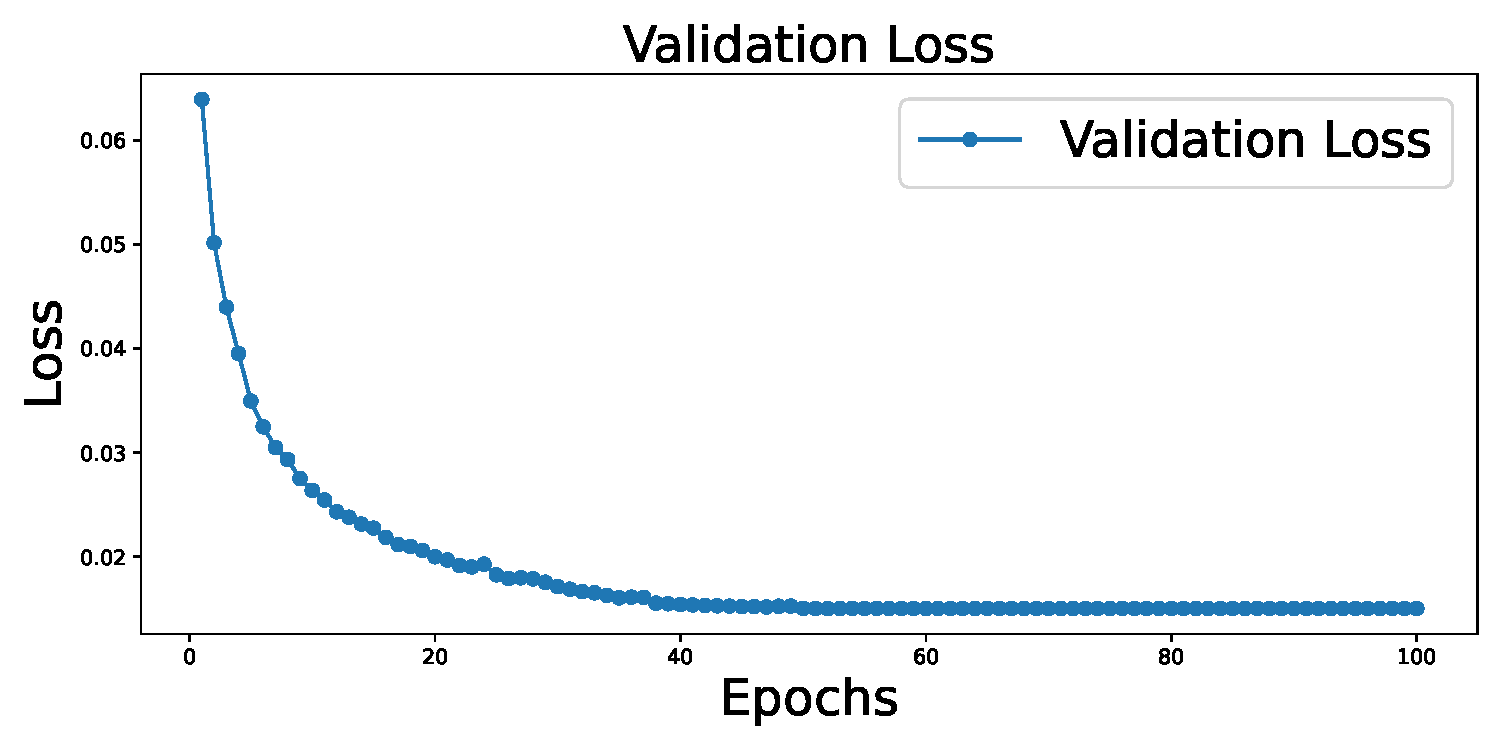
\includegraphics[width=0.7\linewidth]{figures/3d_dcae_training_curve.pdf}
    \caption{Validation Loss Curve for Training of 3D DCAE.}
    \label{fig:3d_dcae_val_loss}
\end{figure}

We developed 3D DCAE by adapting the architecture of 2D DCAE \citep{DCAE} to handle 3D volume inputs. To achieve this, we replaced 2D convolutional layers with 3D convolutional layers and adjusted components such as RMS normalization, batch normalization, \texttt{PixelUnshuffle}, and \texttt{PixelShuffle} to process 3D data effectively. The model was configured with 1 input channel, 1024 latent channels, encoder-decoder width of \texttt{[16, 64, 256, 256, 1024, 1024]}, and encoder-decoder depth of \texttt{[0, 2, 2, 5, 5, 5]}, to make the same compression ratio as the 2D DCAE.

For training, we utilized a dataset of 8,178 subjects from the UK-Biobank, splitting it into training and validation sets with a 9:1 ratio and stratification based on sex and age. The model was trained for 100 epochs with an initial learning rate of $4\times10^{-5}$, which was gradually reduced using \texttt{ReduceLROnPlateau} scheduler. During each epoch, we randomly selected a single fMRI frame from the full set of frames for each subject to train the model. The training process used $\mathcal{L}_2$ reconstruction loss and the AdamW optimizer with a weight decay of $1\times10^{-4}$.

As the training curve in Fig.~\ref{fig:3d_dcae_val_loss} shows, we made every effort to train the 3D DCAE model to achieve the best performance and ensure full convergence, for fair comparison.




\section{Additional Experimental Results}
\subsection{Experiments with Matched $T$}
\label{sec:matchted_t}
We report the performance of {\ours} with $T=20,50$ in \cref{tab:rebuttal1} on HCP and ADHD-200.
The results demonstrate that {\ours} shows comparable performance to SwiFT. Therefore, it proves that {\ours} is able to maintain competitive performance even with a reduced number $T$, highlighting that the performance gain in \cref{tab:main_results} is not solely from the increased $T$, but rather from the effectiveness of the proposed method itself.

\begin{table}[h!]
\caption{Results of experiments with matched $T$ on HCP and ADHD-200.
}
\centering
\resizebox{\columnwidth}{!}{
\centerline{
\begin{tabular}{l|cccccccccccc}
\hline
\multirow{3}{*}{Model} & \multicolumn{9}{c}{HCP}  & \multicolumn{3}{c}{ADHD-200}\\ \cline{2-13} 
 & \multicolumn{3}{c|}{Sex} & \multicolumn{3}{c|}{Age} & \multicolumn{3}{c|}{Intelligence} & \multicolumn{3}{c}{Diagnosis}  \\
 & ACC & AUC & \multicolumn{1}{c|}{F1} & MSE & MAE & \multicolumn{1}{c|}{$\rho$} & MSE & MAE & \multicolumn{1}{c|}{$\rho$} & ACC & AUC & \multicolumn{1}{c}{F1}\\ \hline
SwiFT $(T=20)$ & \textbf{93.1} & 0.978 & \multicolumn{1}{c|}{\textbf{0.937}} & \textbf{0.776} & 0.719 & \multicolumn{1}{c|}{0.450} & 0.940 & 0.782 & \multicolumn{1}{c|}{0.297} & 63.3 & 0.693 & \textbf{0.623} \\
{\ours \ $(T=20)$} & 91.6 & \textbf{0.980} & \multicolumn{1}{c|}{0.923} & 0.784 & \textbf{0.710} & \multicolumn{1}{c|}{\textbf{0.460}} & \textbf{0.866} & \textbf{0.763} & \multicolumn{1}{c|}{\textbf{0.340}} & \textbf{64.4} & \textbf{0.717} & 0.621 \\
\hline

SwiFT $(T=50)$ & 92.2 & 0.972 & \multicolumn{1}{c|}{0.929} & 0.764 & \textbf{0.699} & \multicolumn{1}{c|}{0.460} & \textbf{0.865} & \textbf{0.758} & \multicolumn{1}{c|}{\textbf{0.354}} & 63.9 & 0.701 & \textbf{0.627} \\
{\ours \ $(T=50)$} & \textbf{93.4} & \textbf{0.986} & \multicolumn{1}{c|}{\textbf{0.940}} & \textbf{0.763} & 0.704 & \multicolumn{1}{c|}{\textbf{0.473}} & 0.916 & 0.778 & \multicolumn{1}{c|}{0.334} & \textbf{64.3} & \textbf{0.710} & 0.615 \\

\end{tabular}
}
}
\label{tab:rebuttal1}
\end{table}

\subsection{HBN-Movie Experiments}
\label{sec:hbn}
To test on a more temporally dynamic task, we experimented on Healthy Brain Network (HBN)-Movie \cite{HBN}, which includes 680 subjects and 1,360 fMRI scans where each subject watched two movies. We trained the models to predict which movie was being viewed. As shown in \cref{tab:rebuttal2}, {\ours} achieves performance comparable to SwiFT with the same temporal length $T$, and outperforms with longer $T$, which demonstrates that {\ours} can handle the temporal dynamics of fMRI data.
\begin{table}[h!]
\caption{Results on HBN-Movie.}
\centering
\resizebox{0.6\linewidth}{!}{
\begin{tabular}{l|ccc}
\hline
\multirow{2}{*}{Model} & \multicolumn{3}{c}{HBN-Movie} \\ \cline{2-4} 
 & ACC & AUC & \multicolumn{1}{c}{F1} \\\hline

SwiFT $(T=50)$ & \meanstd{71.7}{4.29} & \meanstd{0.810}{0.040} & \meanstd{0.717}{0.040}\\
{\ours} $(T=50)$ & \meanstd{74.7}{2.38} & \meanstd{0.826}{0.033} & \meanstd{0.750}{0.024} \\
{\ours} $(T=250)$ & \meanstd{\textbf{82.1}}{1.82} & \meanstd{\textbf{0.976}}{0.014} & \meanstd{\textbf{0.847}}{0.015} \\
\hline
\end{tabular}
}
\label{tab:rebuttal2}
\vspace{-0.15in}
\end{table}

\subsection{Axis Aggregation Scheme Variations}
\label{sec:variation_tokenization}
We varied the number of tokens and the latent dimensionality while keeping the total number of values fixed at $27 \times 3072 = 82{,}944$ and setting $T=256$. In other words, we changed the number of tokens that are combined together in the token aggregation step, where combining a larger number of tokens together leads to a larger token dimensionality while reducing the number of total resulting tokens. Since the tokens are only concatenated and rearranged in this step, the total number of values are kept constant $(82{,}944)$. The results are shown in \cref{tab:rebuttal4}. The results indicate that these adjustments do not lead to significant differences in downstream task performance.
 
\begin{table}[h]
\caption{Results on HCP and ADHD-200 with varying axis aggregation schemes.}
\centering
\resizebox{0.8\linewidth}{!}{
\begin{tabular}{l|cc|cccccc}
\hline
\multirow{3}{*}{Model} & \multirow{3}{*}{\# Token} & \multirow{3}{*}{Dim.} & \multicolumn{3}{c}{HCP}  & \multicolumn{3}{c}{ADHD-200}\\ \cline{4-9} 
& & & \multicolumn{3}{c|}{Intelligence} & \multicolumn{3}{c}{Diagnosis}  \\
 & & & MSE & MAE & \multicolumn{1}{c|}{$\rho$} & ACC & AUC & \multicolumn{1}{c}{F1}\\ \hline
 {\ours} & 27 & 3072 & \meanstd{0.835}{0.053} & \meanstd{0.741}{0.028} & \meanstd{0.392}{0.062} & \meanstd{\textbf{65.8}}{3.50} & \meanstd{0.729}{0.029} & \meanstd{0.630}{0.038} \\
 {\ours\ Alt.1} & 9 & 9216 & \meanstd{\textbf{0.814}}{0.044} & \meanstd{\textbf{0.733}}{0.026} & \meanstd{\textbf{0.416}}{0.061} & \meanstd{65.7}{2.74} & \meanstd{0.710}{0.031} & \meanstd{0.632}{0.043} \\
 {\ours\ Alt.2} & 3 & 27648 & \meanstd{0.840}{0.093} & \meanstd{0.736}{0.044} & \meanstd{0.401}{0.035} & \meanstd{65.1}{3.59} & \meanstd{\textbf{0.690}}{0.032} & \meanstd{\textbf{0.636}}{0.042}  \\
\end{tabular}
}
\label{tab:rebuttal4}
\end{table}

\section{Detailed Experimental Results}
\label{sec:detailed_experimental_results}
We provide the results reported in the manuscript with the standard deviation in Tab. ~\ref{tab:std_3}, Tab.~\ref{tab:std_1}, and Tab.~\ref{tab:std_2}.
\begin{table}[ht!]
% \vspace{-0.2in}
\caption{Experimental results with standard deviation on UKB.}
\centering
\resizebox{.85\linewidth}{!}{
\centerline{
\begin{tabular}{l|cccccc}
\hline
\multirow{3}{*}{Method} & \multicolumn{6}{c}{UKB} \\ \cline{2-7}
 & \multicolumn{3}{c|}{Sex} & \multicolumn{3}{c}{Age} \\
 & ACC & AUC & \multicolumn{1}{c|}{F1} & MSE & MAE & \multicolumn{1}{c}{$\rho$} \\ \hline
XGBoost & \meanstd{84.1}{1.7} & \meanstd{0.916}{0.012} & \multicolumn{1}{c|}{\meanstd{0.830}{0.019}} & \meanstd{0.698}{0.013} & \meanstd{0.686}{0.008} & \meanstd{0.553}{0.018}
 \\
BrainNetCNN & \meanstd{91.7}{0.9} & \meanstd{0.969}{0.007} & \multicolumn{1}{c|}{\meanstd{0.912}{0.009}} & \meanstd{0.597}{0.017} & \meanstd{0.618}{0.007} & \meanstd{0.647}{0.012} \\
BNT & \meanstd{92.4}{0.9} & \meanstd{0.980}{0.003} & \multicolumn{1}{c|}{\meanstd{0.919}{0.009}} & \meanstd{0.541}{0.016} & \meanstd{0.588}{0.011} & \meanstd{0.685}{0.011} \\
meanMLP & \meanstd{87.7}{1.8} & \meanstd{0.949}{0.009} & \multicolumn{1}{c|}{\meanstd{0.869}{0.020}} & \meanstd{0.672}{0.031} & \meanstd{0.662}{0.016} & \meanstd{0.586}{0.027}\\
Brain-JEPA & \meanstd{86.8}{0.6} & \meanstd{0.943}{0.004} & \multicolumn{1}{c|}{\meanstd{0.862}{0.007}} & \meanstd{0.688}{0.017} & \meanstd{0.669}{0.008} & \meanstd{0.574}{0.018}\\ \hline
TFF ($T=20$) & \meanstd{98.3}{0.4} & \meanstd{0.998}{0.001} & \multicolumn{1}{c|}{\meanstd{0.982}{0.004}} & \meanstd{0.440}{0.029} & \meanstd{0.525}{0.015} & \meanstd{0.760}{0.015}\\
SwiFT ($T=20$) & \meanstd{97.4}{0.3} & \meanstd{0.998}{0.001} & \multicolumn{1}{c|}{\meanstd{0.972}{0.003}} & \meanstd{0.366}{0.005} & \meanstd{0.480}{0.007} & \meanstd{0.800}{0.004}\\
SwiFT ($T=50$)  & \meanstd{98.1}{0.4} & \meanstd{0.999}{0.001} & \multicolumn{1}{c|}{\meanstd{0.980}{0.005}} & \meanstd{0.364}{0.004} & \meanstd{0.477}{0.005} & \meanstd{0.802}{0.003}\\ \hline
{\ours} ($T=256$) & \meanstd{97.6}{0.2} & \meanstd{0.998}{0.000} & \multicolumn{1}{c|}{\meanstd{0.975}{0.002} }& \meanstd{0.340}{0.011} & \meanstd{0.466}{0.010} & \meanstd{0.814}{0.009}\\ \hline
\end{tabular}
}
}
\label{tab:std_3}
\end{table}

\begin{table}[ht!]
\caption{Experimental results with standard deviation on HCP sex classification and age regression.}
\centering
\resizebox{.85\linewidth}{!}{
\centerline{
\begin{tabular}{l|cccccc}
\hline
\multirow{3}{*}{Method} & \multicolumn{6}{c}{HCP} \\ \cline{2-7}
 & \multicolumn{3}{c|}{Sex} & \multicolumn{3}{c}{Age} \\
 & ACC & AUC & \multicolumn{1}{c|}{F1} & MSE & MAE & \multicolumn{1}{c}{$\rho$} \\ \hline
XGBoost 
& \meanstd{82.2}{2.5} & \meanstd{0.890}{0.028} & \multicolumn{1}{c|}{\meanstd{0.837}{0.025}} & \meanstd{0.859}{0.074} & \meanstd{0.769}{0.033} & \multicolumn{1}{c}{\meanstd{0.296}{0.112}} \\
BrainNetCNN 
& \meanstd{86.3}{4.9} & \meanstd{0.937}{0.027} & \multicolumn{1}{c|}{\meanstd{0.866}{0.049}} & \meanstd{0.847}{0.097} & \meanstd{0.749}{0.040} & \multicolumn{1}{c}{\meanstd{0.372}{0.097}} \\
BNT 
& \meanstd{86.3}{3.0} & \meanstd{0.935}{0.026} & \multicolumn{1}{c|}{\meanstd{0.872}{0.030}} & \meanstd{0.794}{0.051} & \meanstd{0.719}{0.027} & \multicolumn{1}{c}{\meanstd{0.444}{0.055}} \\
meanMLP 
& \meanstd{84.5}{2.5} & \meanstd{0.915}{0.018} & \multicolumn{1}{c|}{\meanstd{0.855}{0.028}} & \meanstd{0.846}{0.056}  & \meanstd{0.751}{0.030}  &   \multicolumn{1}{c}{\meanstd{0.370}{0.087}} \\ 
Brain-JEPA & \meanstd{73.9}{3.2} & \meanstd{0.809}{0.018} & \multicolumn{1}{c|}{\meanstd{0.761}{0.043}} & \meanstd{0.814}{0.037} & \meanstd{0.746}{0.009} &  \meanstd{0.369}{0.046} \\ \hline
TFF ($T=20$) & \meanstd{88.1}{5.0} & \meanstd{0.937}{0.055} & \multicolumn{1}{c|}{\meanstd{0.892}{0.042}} & \meanstd{0.888}{0.062} & \meanstd{0.779}{0.036} & \meanstd{0.246}{0.061}\\
SwiFT ($T=20$) 
% \cite{swift} 
& \meanstd{93.1}{0.5} & \meanstd{0.978}{0.008} & \multicolumn{1}{c|}{\meanstd{0.937}{0.004}} & \meanstd{0.776}{0.043} & \meanstd{0.719}{0.015} & \multicolumn{1}{c}{\meanstd{0.450}{0.031}} \\
SwiFT ($T=50$) 
& \meanstd{92.2}{1.1} & \meanstd{0.972}{0.014} & \multicolumn{1}{c|}{\meanstd{0.929}{0.010}} & \textbf{\meanstd{0.764}{0.092}} & \textbf{\meanstd{0.699}{0.047}} & \multicolumn{1}{c}{\meanstd{0.460}{0.071}} \\ \hline
{\ours} ($T=20$) & \meanstd{91.6}{1.5} & \meanstd{0.980}{0.007} & \meanstd{0.923}{0.014} & \meanstd{0.784}{0.120} & \meanstd{0.710}{0.046} & \meanstd{0.460}{0.087} \\
{\ours} ($T=50$) & \meanstd{93.4}{1.3} & \meanstd{0.986}{0.004} & \multicolumn{1}{c|}{\meanstd{0.940}{0.011}} & \meanstd{0.763}{0.069} & \meanstd{0.704}{0.031} & \multicolumn{1}{c}{\meanstd{0.473}{0.051}} \\

{\ours} ($T=256$) & \meanstd{93.8}{0.9} & \meanstd{0.987}{0.003} & \multicolumn{1}{c|}{\meanstd{0.943}{0.008}} & \meanstd{0.773}{0.077} & \meanstd{0.705}{0.038} & \multicolumn{1}{c}{\meanstd{0.473}{0.053}} \\ \hline\hline
{\ours} (3D DCAE) & \meanstd{92.2}{1.7} & \meanstd{0.973}{0.010} & \multicolumn{1}{c|}{\meanstd{0.929}{0.014}} & \meanstd{0.767}{0.118} & \meanstd{0.693}{0.043} & \multicolumn{1}{c}{\meanstd{0.475}{0.076}} \\ 
{\ours} (FT) & \meanstd{95.3}{1.3} & \meanstd{0.986}{0.005} & \multicolumn{1}{c|}{\meanstd{0.958}{0.011}} & \meanstd{0.650}{0.045} & \meanstd{0.655}{0.024} & \meanstd{0.552}{0.032}\\\hline
\end{tabular}
}
}
\label{tab:std_1}
\end{table}
\begin{table}[ht!]
\caption{Main experimental results with standard deviation on HCP intelligence regression and ADHD diagnosis.}
\centering
\resizebox{.85\linewidth}{!}{
\centerline{
\begin{tabular}{l|ccc|ccc}
\hline
\multirow{3}{*}{Method} & \multicolumn{3}{c}{HCP} & \multicolumn{3}{c}{ADHD-200} \\ \cline{2-7}
 & \multicolumn{3}{c|}{Intelligence} & \multicolumn{3}{c}{Diagnosis} \\
 & MSE & MAE & $\rho$ & ACC & AUC & F1 \\ \hline
XGBoost 
& \meanstd{0.908}{0.054} & \meanstd{0.779}{0.023} & \meanstd{0.292}{0.099} & \meanstd{62.3}{2.5} & \meanstd{0.650}{0.036} & \meanstd{0.555}{0.031} \\
BrainNetCNN 
& \meanstd{0.967}{0.119} & \meanstd{0.788}{0.044} & \meanstd{0.286}{0.112} & \meanstd{59.2}{10.7} & \meanstd{0.640}{0.095} & \meanstd{0.545}{0.118} \\
BNT 
& \meanstd{0.920}{0.092} & \meanstd{0.778}{0.054} & \meanstd{0.318}{0.083} & \meanstd{63.6}{5.4} & \meanstd{0.677}{0.062} & \meanstd{0.624}{0.057} \\
meanMLP 
& \meanstd{0.887}{0.076}& \meanstd{0.767}{0.028} & \meanstd{0.340}{0.045} & \meanstd{56.8}{6.8} & \meanstd{0.617}{0.067} & \meanstd{0.532}{0.095} \\ 
Brain-JEPA &\meanstd{0.959}{0.091} &\meanstd{0.799}{0.033} &\multicolumn{1}{c|}{\meanstd{0.171}{0.051}} & -- & -- & -- \\ \hline
TFF ($T=20$) & \meanstd{0.898}{0.022} & \meanstd{0.767}{0.018} & \multicolumn{1}{c|}{\meanstd{0.312}{0.088}} & \meanstd{63.3}{2.3} & \meanstd{0.700}{0.028} & \meanstd{0.608}{0.030}\\
SwiFT ($T=20$) 
& \meanstd{0.940}{0.111} & \meanstd{0.782}{0.044} & \meanstd{0.297}{0.080} & \meanstd{63.3}{3.7} & \meanstd{0.693}{0.030} & \meanstd{0.623}{0.033} \\
SwiFT ($T=50$) 
& \meanstd{0.865}{0.093} & \meanstd{0.758}{0.046} & \meanstd{0.354}{0.070} & \meanstd{63.9}{3.2} & \meanstd{0.701}{0.032} & \meanstd{0.627}{0.030} \\ \hline
{\ours} ($T=20$) & \meanstd{0.866}{0.074} & \meanstd{0.763}{0.042} & \meanstd{0.340}{0.045} & \meanstd{64.4}{3.0} & \meanstd{0.717}{0.020} & \meanstd{0.621}{0.039}\\
{\ours} ($T=50$) & \meanstd{0.916}{0.155} & \meanstd{0.778}{0.063} & \meanstd{0.334}{0.102} & \meanstd{64.3}{2.8} & \meanstd{0.710}{0.021} & \meanstd{0.615}{0.037} \\

{\ours} ($T=256$) & \meanstd{0.835}{0.053} & \meanstd{0.741}{0.028} & \meanstd{0.392}{0.062} & \meanstd{65.8}{3.5} & \meanstd{0.729}{0.029} & \meanstd{0.630}{0.038} \\ \hline\hline
{\ours} (3D DCAE) & \meanstd{0.869}{0.077} & \meanstd{0.755}{0.032} & \meanstd{0.387}{0.078} & \meanstd{65.8}{1.7} & \meanstd{0.711}{0.026} & \meanstd{0.644}{0.022} \\ 
{\ours} (FT) & \meanstd{0.796}{0.051} & \meanstd{0.732}{0.028} & \meanstd{0.435}{0.046} & - & - & - \\\hline

\end{tabular}
}
\label{tab:std_2}
}
\end{table}

\section{Detailed Data Description}
\label{sec:detailed_data_description}
We provide a detailed description of each dataset used in our study in Tab.~\ref{tab:demographics}.

\begin{table}[ht]
  \centering
  \caption{Demographic information of the datasets used in our study}
  \label{tab:demographics}
  \begin{tabular}{l|ccc}
  \hline
    Category            & UKB & HCP              & ADHD
    -200          \\ \hline
    Number of subjects  & 8,178 & 1,061             & 533              \\
    Sex \\
    \hspace{1em}Male, n (\%)       & 4,295 (52.5\%) & 488 (46.0\%)     & 207 (38.8\%)     \\
    \hspace{1em}Female, n (\%)     & 3,883 (47.5\%) & 573 (54.0\%)     & 325 (61.0\%)     \\
    \hspace{1em}N/A, n (\%)         & -- & --               & 1 (0.2\%)        \\
    Age (years) & \meanstd{54.98}{7.53} & \meanstd{28.79}{3.70} & \meanstd{11.94}{3.40} \\
    Intelligence & -- & \meanstd{113.32}{20.50} & -- \\
    Diagnosed, n (\%)  &-- & --               & 236 (44.3\%)     \\ \hline
  \end{tabular}
\end{table}